% Options for packages loaded elsewhere
\PassOptionsToPackage{unicode}{hyperref}
\PassOptionsToPackage{hyphens}{url}
\documentclass[
]{article}
\usepackage{xcolor}
\usepackage[margin=1in]{geometry}
\usepackage{amsmath,amssymb}
\setcounter{secnumdepth}{-\maxdimen} % remove section numbering
\usepackage{iftex}
\ifPDFTeX
  \usepackage[T1]{fontenc}
  \usepackage[utf8]{inputenc}
  \usepackage{textcomp} % provide euro and other symbols
\else % if luatex or xetex
  \usepackage{unicode-math} % this also loads fontspec
  \defaultfontfeatures{Scale=MatchLowercase}
  \defaultfontfeatures[\rmfamily]{Ligatures=TeX,Scale=1}
\fi
\usepackage{lmodern}
\ifPDFTeX\else
  % xetex/luatex font selection
\fi
% Use upquote if available, for straight quotes in verbatim environments
\IfFileExists{upquote.sty}{\usepackage{upquote}}{}
\IfFileExists{microtype.sty}{% use microtype if available
  \usepackage[]{microtype}
  \UseMicrotypeSet[protrusion]{basicmath} % disable protrusion for tt fonts
}{}
\makeatletter
\@ifundefined{KOMAClassName}{% if non-KOMA class
  \IfFileExists{parskip.sty}{%
    \usepackage{parskip}
  }{% else
    \setlength{\parindent}{0pt}
    \setlength{\parskip}{6pt plus 2pt minus 1pt}}
}{% if KOMA class
  \KOMAoptions{parskip=half}}
\makeatother
\usepackage{longtable,booktabs,array}
\usepackage{calc} % for calculating minipage widths
% Correct order of tables after \paragraph or \subparagraph
\usepackage{etoolbox}
\makeatletter
\patchcmd\longtable{\par}{\if@noskipsec\mbox{}\fi\par}{}{}
\makeatother
% Allow footnotes in longtable head/foot
\IfFileExists{footnotehyper.sty}{\usepackage{footnotehyper}}{\usepackage{footnote}}
\makesavenoteenv{longtable}
\usepackage{graphicx}
\makeatletter
\newsavebox\pandoc@box
\newcommand*\pandocbounded[1]{% scales image to fit in text height/width
  \sbox\pandoc@box{#1}%
  \Gscale@div\@tempa{\textheight}{\dimexpr\ht\pandoc@box+\dp\pandoc@box\relax}%
  \Gscale@div\@tempb{\linewidth}{\wd\pandoc@box}%
  \ifdim\@tempb\p@<\@tempa\p@\let\@tempa\@tempb\fi% select the smaller of both
  \ifdim\@tempa\p@<\p@\scalebox{\@tempa}{\usebox\pandoc@box}%
  \else\usebox{\pandoc@box}%
  \fi%
}
% Set default figure placement to htbp
\def\fps@figure{htbp}
\makeatother
\setlength{\emergencystretch}{3em} % prevent overfull lines
\providecommand{\tightlist}{%
  \setlength{\itemsep}{0pt}\setlength{\parskip}{0pt}}
\usepackage{bookmark}
\IfFileExists{xurl.sty}{\usepackage{xurl}}{} % add URL line breaks if available
\urlstyle{same}
\hypersetup{
  pdftitle={Habitat quelques chiffres},
  pdfauthor={B. Maranget},
  hidelinks,
  pdfcreator={LaTeX via pandoc}}

\title{Habitat quelques chiffres}
\author{B. Maranget}
\date{2026-04-07}

\begin{document}
\maketitle

{
\setcounter{tocdepth}{2}
\tableofcontents
}
\section{Objet}\label{objet}

La direction de l'habitat cherche à avoir quelques chiffres repères.

\section{Population totale}\label{population-totale}

\subsection{Evolution : chiffres insee}\label{evolution-chiffres-insee}

\url{https://www.insee.fr/fr/statistiques/3698339\#consulter}

Il existe une tendance à la baisse depuis 2019 (de 55 000 à 50 000
environ).

\pandocbounded{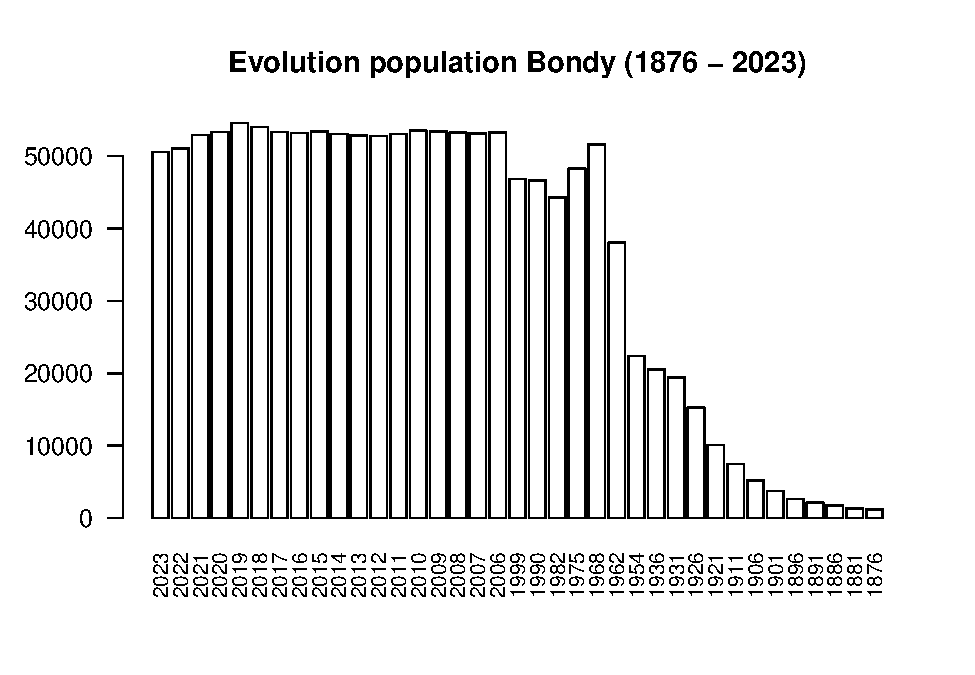
\includegraphics[keepaspectratio]{habitatChiffres_files/figure-latex/unnamed-chunk-3-1.pdf}}
\pandocbounded{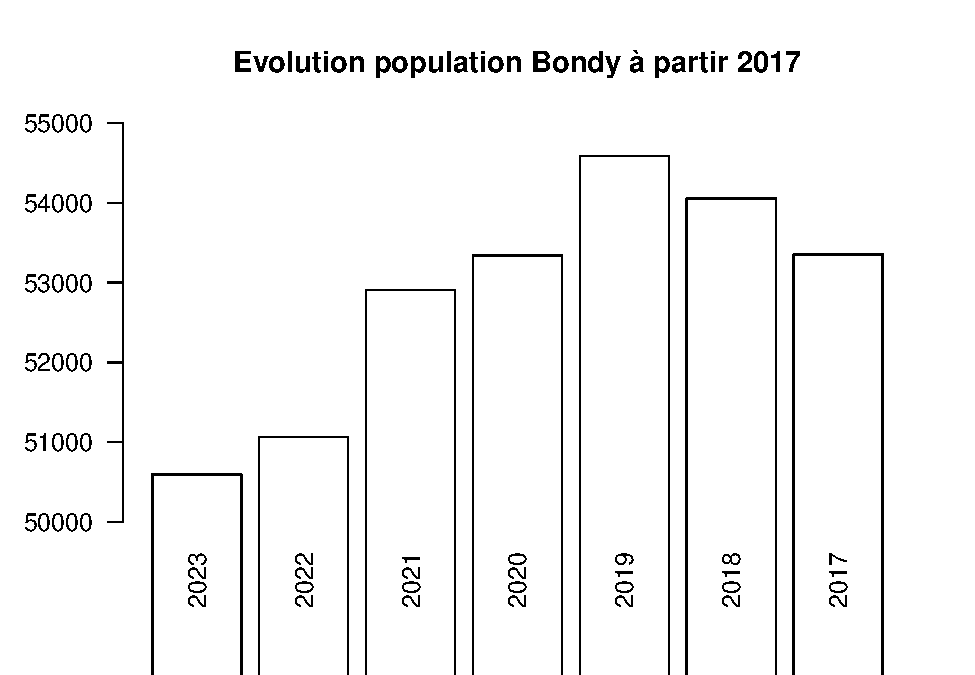
\includegraphics[keepaspectratio]{habitatChiffres_files/figure-latex/unnamed-chunk-3-2.pdf}}

\begin{longtable}[]{@{}rr@{}}
\toprule\noalign{}
année & nb \\
\midrule\noalign{}
\endhead
\bottomrule\noalign{}
\endlastfoot
2023 & 50595 \\
2022 & 51066 \\
2021 & 52905 \\
2020 & 53342 \\
2019 & 54587 \\
2018 & 54055 \\
2017 & 53353 \\
\end{longtable}

\subsection{Ril 2025}\label{ril-2025}

Le ril (Répertoire Immeuble Localisé) indique le nombre d'habitats, même
en multipliant par 2, le chiffre obtenu est supérieur aux chiffres
insee.

\begin{longtable}[]{@{}
  >{\raggedleft\arraybackslash}p{(\linewidth - 12\tabcolsep) * \real{0.0745}}
  >{\raggedright\arraybackslash}p{(\linewidth - 12\tabcolsep) * \real{0.1170}}
  >{\raggedright\arraybackslash}p{(\linewidth - 12\tabcolsep) * \real{0.1170}}
  >{\raggedright\arraybackslash}p{(\linewidth - 12\tabcolsep) * \real{0.1064}}
  >{\raggedright\arraybackslash}p{(\linewidth - 12\tabcolsep) * \real{0.2340}}
  >{\raggedleft\arraybackslash}p{(\linewidth - 12\tabcolsep) * \real{0.1809}}
  >{\raggedright\arraybackslash}p{(\linewidth - 12\tabcolsep) * \real{0.1702}}@{}}
\toprule\noalign{}
\begin{minipage}[b]{\linewidth}\raggedleft
numero
\end{minipage} & \begin{minipage}[b]{\linewidth}\raggedright
repetition
\end{minipage} & \begin{minipage}[b]{\linewidth}\raggedright
complement
\end{minipage} & \begin{minipage}[b]{\linewidth}\raggedright
type\_voie
\end{minipage} & \begin{minipage}[b]{\linewidth}\raggedright
libelle
\end{minipage} & \begin{minipage}[b]{\linewidth}\raggedleft
nombre\_logements
\end{minipage} & \begin{minipage}[b]{\linewidth}\raggedright
numero\_parcelle
\end{minipage} \\
\midrule\noalign{}
\endhead
\bottomrule\noalign{}
\endlastfoot
19 & & & ALL & DE LA VILLA JEANNETTE & 1 & AN0055 \\
2 & & BAT D & R & BENOITE GROULT & 29 & 0H0415 \\
26 & & & R & DU BON AIR & 2 & 0B0211 \\
25 & & & R & DU CYCLE & 1 & 0T0029 \\
3 & & & R & BORDIER & 6 & AL0118 \\
5 & & & ALL & ANNE SYLVESTRE & 1 & 0A0378 \\
\end{longtable}

\begin{verbatim}
## [1] 56150
\end{verbatim}

A noter, l'estimation à partir du RIL donne plus d'habitants que le
chiffre INSEE de 2023

\section{Indicateurs sociaux globaux}\label{indicateurs-sociaux-globaux}

\subsection{Seuil de pauvreté}\label{seuil-de-pauvretuxe9}

\begin{longtable}[]{@{}
  >{\raggedright\arraybackslash}p{(\linewidth - 2\tabcolsep) * \real{0.9114}}
  >{\raggedleft\arraybackslash}p{(\linewidth - 2\tabcolsep) * \real{0.0886}}@{}}
\toprule\noalign{}
\begin{minipage}[b]{\linewidth}\raggedright
Mesures.filosofi
\end{minipage} & \begin{minipage}[b]{\linewidth}\raggedleft
Valeur
\end{minipage} \\
\midrule\noalign{}
\endhead
\bottomrule\noalign{}
\endlastfoot
Taux de pauvreté (en \%) au seuil de 60 \% de la médiane du niveau de
vie & 34 \\
\end{longtable}

\subsection{Logements sociaux}\label{logements-sociaux}

\pandocbounded{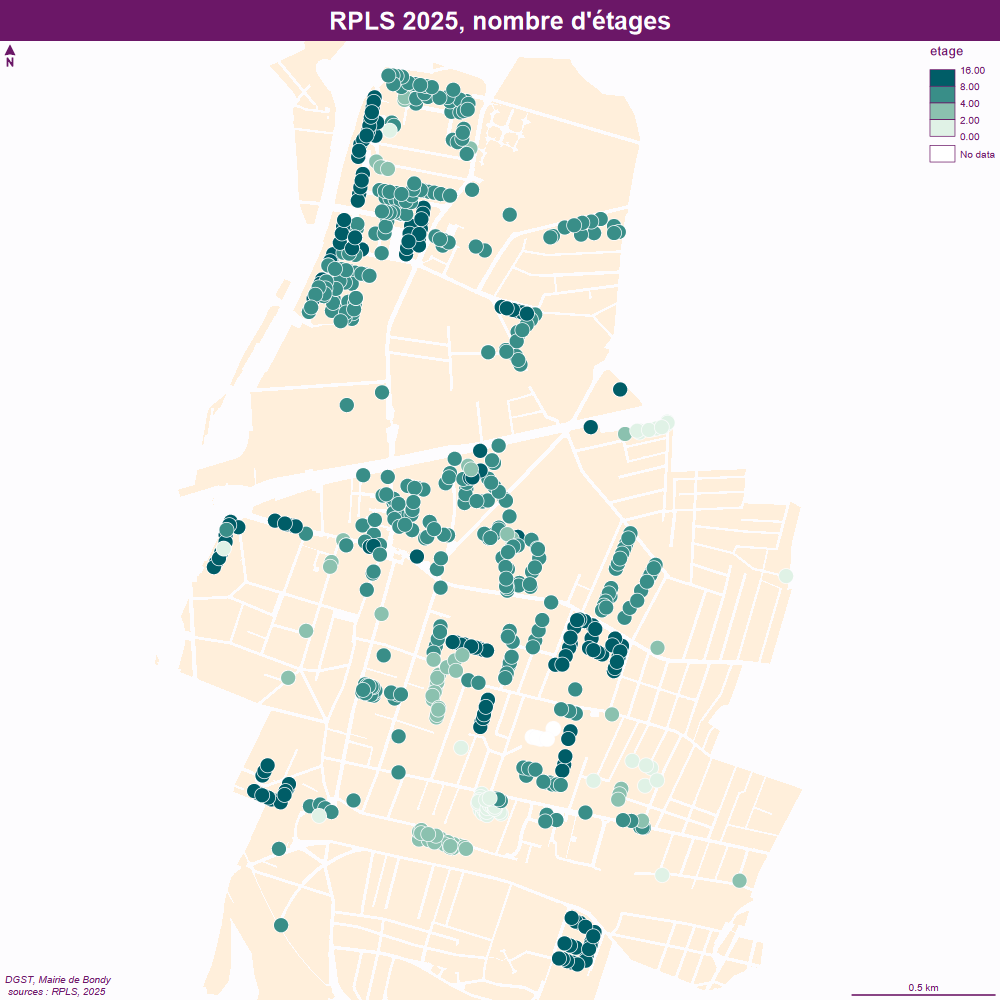
\includegraphics[keepaspectratio]{../img/RPLS2025.png}}

Nb de logements sociaux

\begin{verbatim}
## [1] 108788
\end{verbatim}

\begin{longtable}[]{@{}lr@{}}
\toprule\noalign{}
Nb étages & Nb immeubles \\
\midrule\noalign{}
\endhead
\bottomrule\noalign{}
\endlastfoot
0 & 48 \\
1 & 2 \\
2 & 11 \\
3 & 56 \\
4 & 180 \\
5 & 149 \\
6 & 29 \\
7 & 2 \\
8 & 18 \\
9 & 37 \\
10 & 79 \\
12 & 39 \\
15 & 1 \\
18 & 5 \\
\end{longtable}

A noter, Marx Dormoy / ZAC de l'Ourcq / Sablière / allée Laffargue

\section{Typologie occupation
logements}\label{typologie-occupation-logements}

En pourcentage du nb de logement total

\begin{longtable}[]{@{}
  >{\raggedleft\arraybackslash}p{(\linewidth - 12\tabcolsep) * \real{0.1733}}
  >{\raggedleft\arraybackslash}p{(\linewidth - 12\tabcolsep) * \real{0.2133}}
  >{\raggedleft\arraybackslash}p{(\linewidth - 12\tabcolsep) * \real{0.0533}}
  >{\raggedleft\arraybackslash}p{(\linewidth - 12\tabcolsep) * \real{0.1333}}
  >{\raggedleft\arraybackslash}p{(\linewidth - 12\tabcolsep) * \real{0.1067}}
  >{\raggedleft\arraybackslash}p{(\linewidth - 12\tabcolsep) * \real{0.1067}}
  >{\raggedleft\arraybackslash}p{(\linewidth - 12\tabcolsep) * \real{0.2133}}@{}}
\toprule\noalign{}
\begin{minipage}[b]{\linewidth}\raggedleft
proprio 2022
\end{minipage} & \begin{minipage}[b]{\linewidth}\raggedleft
Locataires 2022
\end{minipage} & \begin{minipage}[b]{\linewidth}\raggedleft
HLM
\end{minipage} & \begin{minipage}[b]{\linewidth}\raggedleft
RPLS 2023
\end{minipage} & \begin{minipage}[b]{\linewidth}\raggedleft
RP 2022
\end{minipage} & \begin{minipage}[b]{\linewidth}\raggedleft
vacants
\end{minipage} & \begin{minipage}[b]{\linewidth}\raggedleft
vacants 2 ans +
\end{minipage} \\
\midrule\noalign{}
\endhead
\bottomrule\noalign{}
\endlastfoot
35 & 20 & 34 & 44 & 89 & 10 & 2 \\
\end{longtable}

source : ANCT

\section{Disparités territoriales}\label{disparituxe9s-territoriales}

Croisement de deux sources Insee Filosofi (tx pauvreté) et ANCT (rpls)

\% de logement social / \% de la population sous le seuil de pauvreté

Plus le chiffre est élevé, plus l'offre en logement social répond aux
besoins de la taille de la population modeste.

\begin{longtable}[]{@{}lr@{}}
\toprule\noalign{}
ville & rapport \\
\midrule\noalign{}
\endhead
\bottomrule\noalign{}
\endlastfoot
Bagnolet & 70 \\
Bondy & 77 \\
Le Pré Saint Gervais & 56 \\
Romainville & 71 \\
\end{longtable}

Cartographie

\pandocbounded{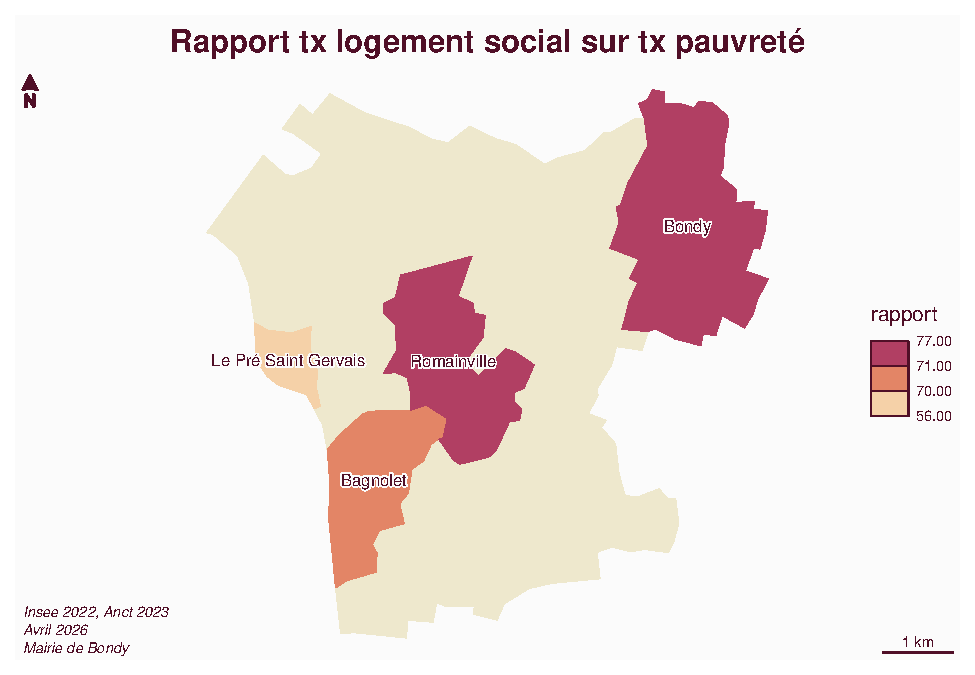
\includegraphics[keepaspectratio]{habitatChiffres_files/figure-latex/unnamed-chunk-12-1.pdf}}

\section{Traitement des demandes de logement
social}\label{traitement-des-demandes-de-logement-social}

\url{https://www.demande-logement-social.gouv.fr/offresParCommune.afficher}

\subsection{Nombre de demandes}\label{nombre-de-demandes}

\begin{verbatim}
## [1] "4693 demandes en attente sur Bondy"
\end{verbatim}

\% demandeurs en PLAI

\subsection{PLAI}\label{plai}

Pas de donnée pour les dossiers en attente, dans le RPLS, la variable
CUS = 11 indique le nombre de PLAI sur le parc social

\begin{verbatim}
## 
##   10   13   14   16 <NA> 
##   87  212  287   21 9099
\end{verbatim}

\pandocbounded{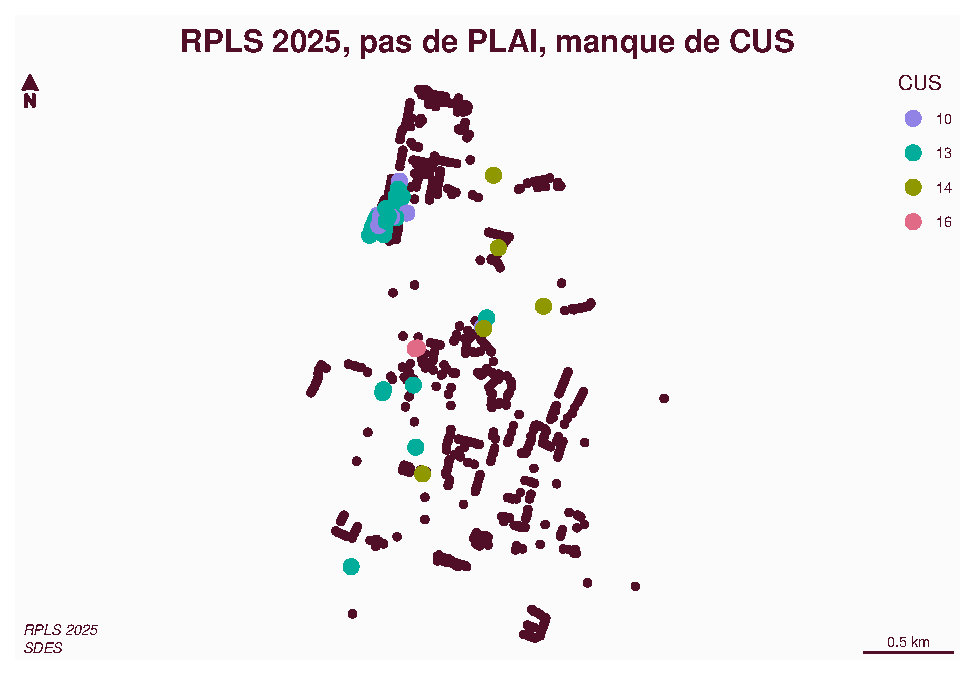
\includegraphics[keepaspectratio]{habitatChiffres_files/figure-latex/unnamed-chunk-14-1.pdf}}

CUS 10 = PLA d'intégration

CUS 13 = 13.PLUS

CUS 14 = PLS / PPLS / PLA CFF

CUS 16 = 16.PLI

\subsection{DALO (au dpt)}\label{dalo-au-dpt}

\begin{verbatim}
##              dpt nb.favorable nb.réalité
## 6 Seine St Denis         4646       2379
\end{verbatim}

\subsection{Logement indigne (au dpt)}\label{logement-indigne-au-dpt}

\begin{verbatim}
## 
##                         Procédure d'insalubrité remédiable ou irrémédiable 
##                                                                        429 
##               Procédure d'urgence d'insalubrité remédiable ou irrémédiable 
##                                                                         17 
##                  Procédure désordre ponctuel présentant un danger imminent 
##                                                                        125 
## Procédure relative aux locaux dangereux par l'utilisation qui en est faite 
##                                                                         32 
##                             Procédure relative aux locaux en suroccupation 
##                                                                         25 
##                     Procédure relative aux locaux impropres à l'habitation 
##                                                                        311 
##                                                       Procédure saturnisme 
##                                                                        572
\end{verbatim}

\pandocbounded{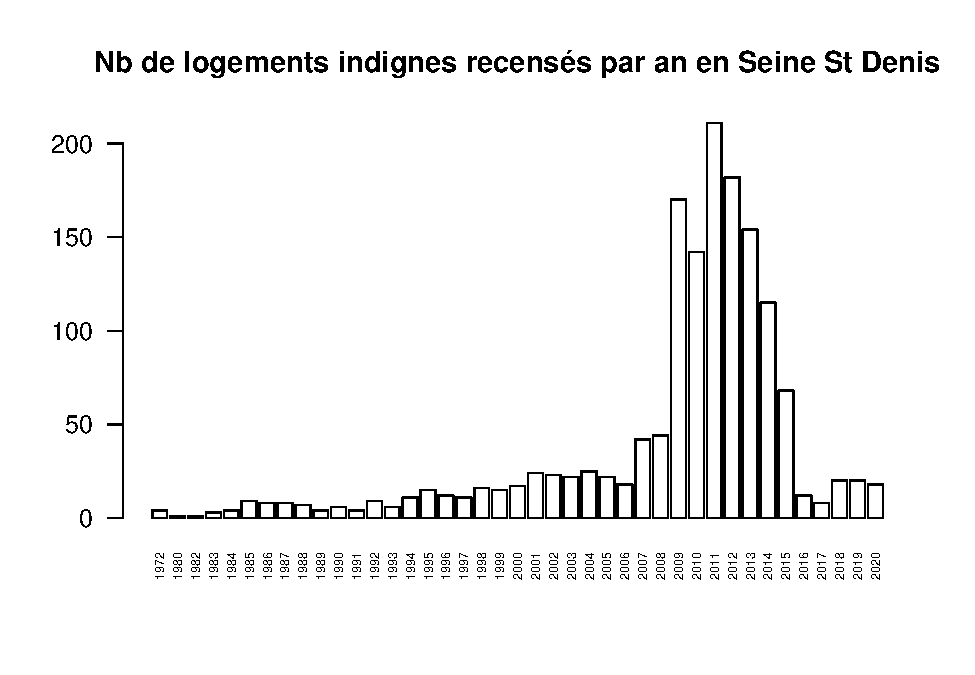
\includegraphics[keepaspectratio]{habitatChiffres_files/figure-latex/unnamed-chunk-16-1.pdf}}

\end{document}
